\documentclass[10pt]{article}

\usepackage[utf8]{inputenc}
\usepackage{amsmath}
\usepackage{amsfonts}
\usepackage{graphicx}
\usepackage{geometry}
\usepackage{fancyhdr}
\usepackage{multicol}
\usepackage{hyperref}
\usepackage{titlesec}
\usepackage{subcaption}
\usepackage{float}

\geometry{margin=1in}

\title{Taming the LLaMA: Fine-Tuning a 3B Parameter Model for Artificial Intelegence and Machine Learning}

\author{
        \begin{minipage}{0.3\textwidth}
            \centering
            Arlo Steyn\\
            24713848
        \end{minipage}%  
    \hfill
        \begin{minipage}{0.3\textwidth}
            \centering
            Andre van der Merwe\\
            24923273
        \end{minipage}%
    \hfill
        \begin{minipage}{0.3\textwidth}
            \centering
            Stephan Delport\\
            24710083
        \end{minipage}%
}

\begin{document}

\maketitle

\section{Introduction}
Large language models (LLMs) have revolutionized natural language processing tasks,
which offers advanced capabilities in generating human like responses. This project
aimed to fine-tune LLaMA, a 3 billion parameter model on a scraped dataset that contains
questions and answers related to data science, artificial intelligence, and machine learning.
By using Kaggle's free GPU resources, we successfully fine-tuned two models: one trained on
the full dataset and another on a subset of the data, allowing us to compare their performance
in generating accurate and contextually relevant answers. This report outlines the steps taken
in data collection, model fine-tuning, and performance evaluation.

\section{Web Scraping Cross Validated}

This section of the report provides an overview of the Cross Validated website,
details about the scraped data, and the tools used in the scraping process.

\subsection{Overview of Cross Validated}

With the ever-expanding fields of statistics and machine learning (ML), it is hard to keep up with all of
the new ideas and models being introduced.
Cross Validated \cite{stackexchange}, part of the Stack Exchange network, hosts a specialised question-and-answer platform
dedicated to topics such as:
\begin{itemize}
    \item Statistics
    \item Machine learning
    \item Data analysis
    \item Data mining
    \item Data visualisation
\end{itemize}
Cross Validated provides a community-driven environment for professionals and enthusiasts to ask and answer
questions, share knowledge and discuss best practices in these fields \cite{stackexchange-tour}.

\subsection{Data Overview}

The objective we wanted to complete was to gather any meaningful insights on common challenges
faced by data scientists and optimal solutions to these challenges. Cross Validated offered us a wealth of
information, more than sufficient to achieve our goal.

We scraped 39,668 of the highest-voted questions and their corresponding highest-voted answer from Cross Validated.
Only the text bodies of each question and answer were scraped to ensure the data contained no personal information.
We strictly wanted to focus on a model that only generates text. Therefore, we excluded any questions or answers
which contained code blocks in the body of the text.

\subsection{Tools and Techniques for Data Scraping}

Python and the Beautifulsoup4 library \cite{beautifulsoup} was utilised to scrape the question-and-answer pairs
from Cross Validated. Stack Exchange enforces several throttling limits based on the Internet Protocol (IP)
address of the user \cite{stackexchange-throttle}. If a single IP exceeds 30 requests per second, 
any additional requests will be dropped and the user's IP will be temporarily blocked. To prevent our scraper from
violating this throttle, we implemented an exponential backoff function, which reduced the likelihood of
triggering the throttle and ensuring smoother data retrieval.

All question-and-answer pairs were scraped in batches of 5,000 observations and subsequently
stored in their respective Javascript object notation (JSON) files.

\section{Ethics Regarding Web Scraping}

This section of the report focuses on the ethical considerations we examined prior to scraping our data.
While scraping information from the web can be extremely useful, especially for building a large language
model, the ethical concerns should always be addressed. This includes intellectual property, personal
property and informed consent. There is a fine balance between balancing respect for privacy and the
utility of web scraping.

\subsection{Intellectual Property}

There are laws that protect websites such as copyright and one should step carefully not to unintentionally
break a law. It is important therefore to read the sites terms of service to make
sure you don't use any data you are not allowed to \cite{stackexchange-terms}.

\subsection{Personal Property}
Personal information is protected by the protection of personal information (POPI) act and it is usually of
your best interest to not scrape any personal information from a website. If personal information does slip
through one should pseudonymise and anonymise the data. 

\subsection{Informed Consent}

Even if the data is publicly available it does not mean you have the right to use it. You should ask
beforehand if you are allowed to use the data and for what purposes.
There are steps you can follow to help you ethically scrape data:
\begin{itemize}
    \item Targeted scraping: Only scrape the data that you need, do not scrape extra information such as personal information.
    \item Legal compliance: Ensure that you follow the websites terms of service as well as any other laws.
    \item Respecting data ownership: Online data still belongs to the person who posted it, make sure you use the data in a way that respects their rights.
\end{itemize}

\section{Wrangling The Scraped Data}

This section of the report focuses on cleaning, normalising and saving the scraped data
by applying wrangling techniques.

\subsection{Data Cleaning}

The scraped data was cleaned to ensure there are no irrelevant text in the data. Questions that
were closed or locked by the site admins contained a post notification board, which was removed
from the data by utilising beautifulsoup4. Any Hypertext Markup Language (HTML) tags that contained relevant text was then kept
in all of the question-and-answer pairs. These HTML tags were: $<$p$>$, $<$code$>$, $<$a$>$, $<$ol$>$, $<$li$>$, $<$ul$>$,
$<$strong$>$, $<$b$>$, $<$i$>$, $<$u$>$, $<$mark$>$, $<$small$>$, $<$sub$>$, $<$sup$>$, $<$span$>$, $<$table$>$.

From these remaining HTML tags, the text were stripped away and we were left with only the
text of all of the question-and-answer pairs.

\subsection{Text Normalisation, Structuring and Saving the Data}

From the cleaned body text of the questions-and-answer pairs, some characters were
encoded as Unicode characters. These characters were then encoded to either American Standard Code for Information Interchange (ASCII)
characters if they had an ASCII index or to HTML entities if they did not.

The data was then structured into a list of dictionaries, categorising questions as the role of the "user"
and the answers as the role of the "assistant". This format was used to comply with the format required by
the LLaMa model.

The list of dictionaries, which contains the cleaned, normalised and structured data, was then saved to
a new JSON file.

\section{LLaMA Model Overview and Fine-tuning Process}

We used the large language model meta AI (LLaMA) model, specifically the 3-billion parameter version,
which is part of a family of transformer-based models \cite{llama3herd}. Llama is an open source LLM provided by Meta
and we specifically used the LLaMA-3B-Instruct model for question-and-answering. LLaMA is designed for natural
language processing tasks, and its architecture follows a standard decoder-only transformer,
making it suitable for autoregressive text generation. This model is ideal for tasks like question answering,
summarisation, and dialogue generation, but also has many other abilities and applications.

\subsection{Model Architecture}
The LLaMA model is built on the transformer architecture, which uses self attention mechanisms to process input
sequences and generate output. It is also autoregressive which means that it generates text one token at a time,
using previously generated tokens to predict the next one.

Key components of the LLaMA model architecture include:
\begin{itemize}
    \item Multi-Head Self-Attention: This allows the model to focus on different parts of the input sequence at the same time, which allows it to capture relationships between words across long sequences.
    \item Attention Heads: 32 heads per layer
    \item Attention Head Dimension: 128 dimensions per head
    \item Feed-Forward Networks (FFN): These are fully connected layers that transform the output of the self-attention mechanism.
    \item Feed-Forward Network Dimension: 11008 units (intermediate layer)
    \item Model Size: 3 billion parameters
    \item Number of Layers: 32 transformer layers
    \item Hidden Size: 4096 hidden units per layer
    \item Positional Encoding: Rotary positional encodings (RoPE)
    \item Layer Normalisation: Applied before self-attention and feed-forward layers
\end{itemize}

\subsection{Pre-Trained Weights and Dataset}

The pre-trained weights for the LLaMA model were obtained from the Unsloth repository, which
provided a specialised model version fine-tuned for question-and-answer and conversational tasks.
The initial pre-training of LLaMA was done on a large corpus of diverse text, including books,
research papers, and web data. This gives the model a strong foundation in understanding complex
language structures and domain specific terminology.

We fine-tuned the model using a custom dataset of 39,668 question-and-answer pairs, which were scraped
from `Cross Validated' which focused on data science, artificial intelligence (AI), and ML topics.
These questions ranged from simple definitions to more complex conceptual explanations. Fine-tuning allowed the
model to better capture the complexity of these technical subjects, which makes it more accurate in responding and
understanding to domain specific applications.

\subsection{Fine-Tuning Process}

The version of LLaMA we used was fine-tuned for question-and-answering tasks, making it ideal for providing answers
to questions related to data science, AI, and ML.
Fine-tuning was performed using the Low-Rank Adaptation (LoRA) technique, which allows for efficient fine-tuning
of large models by freezing most of the pre-trained model parameters and only updating a small subset of parameters.
This drastically reduces the computational resources required, and also still achives high accuracy. We used
a combination of gradient accumulation and batch processing to handle the relatively large dataset size during
the fine-tuning phase.

The fine-tuning process involved adjusting several hyperparameters, including:
\begin{itemize}
    \item Learning rate: Set to 2e-4 for optimal convergence without overfitting.
    \item Batch size: A batch size of 4 per GPU was used to maximise the use of available memory.
    \item Gradient accumulation: This was set to 4, allowing larger effective batch sizes without exceeding memory limits.
\end{itemize}
We also used 4-bit quantization during training to optimise memory usage, enabling us to fine-tune the model on hardware with limited GPU resources.

\section{Quantization and Tokenization}

Tokenization creates tokens for words or subwords in a text.
We used Byte-Pair Encoding (BPE), which splits long complex words into smaller
words which is then easier for the model to understand. The tokens are then mapped to numerical
representations. Each token then has the meaning in the context of which it is used. The model
can then make predictions from these tokens.

Quantization is the process of simplifying machine learning models by reducing the
precision of the numbers they use for weights and activations. Normally they use 32-bit
floating-point numbers, which is demanding on memory and processing power. By switching to
lower precision, such as 8-bit or 4-bit numbers, the model is made faster and more
memory-efficient without affecting accuracy too much. In this project, we employed
\textit{4-bit quantization} during the fine-tuning stage. This method allowed it to
run on hardware with limited GPU resources when fine-tuning our model.

\section{UnSloth Optimisation}

Fine-tuning is devined as the process of updating the actual "brains" of the language model
through back-propagation. But, finetuning can get very slow and very resource intensive.
UnSloth Optimisation helps to optimise the process of finetuning our model.

UnSloth is a fine-tuning framework designed to enhance productivity by streamlining the
process of adapting LLM like Llama-3.2. UnSloth makes fine-tuning
LLM \cite{unslothdocs}:
\begin{itemize}
    \item 2 times faster
    \item Use 70\% less memory
    \item Automates hyperparameter tuning
    \item Maintains model accuracy
\end{itemize}

We used UnSloth optimisation to optimise the fine-tuning process of our LLaMa model \cite{unslothfine-tune}.
UnSloth applies the following techniques to ensure the fine-tuning
of our model is optimised as much as possible:
\begin{itemize}
    \item Layer-freezing: reduces computation, by only fine-tuning specific layers.
    \item Gradient checkpointing: recomputes activations, which lowers memory usage.
    \item Dynamic hyperparameter tuning: Automatically adjusts the hyperparameters during the fine-tuning process.
    \item Efficient data loading: Speeds up fine-tuning with optimised data handling.
\end{itemize}

\section{Implementation}

This section introduces the final models after fine-tuning the LLaMa-3.2 model on our scraped data.
We wanted to explore if more data is always better for training or fine-tuning a model.

We constructed 2 models, the first model fine-tuned the original model on the full dataset of
39,668 question-and-answer pairs for one epoch and the second model fine-tuned the original model
on the 10,000 highest-voted question-and-answer pairs for three epochs. Both of the models took
approximately 12 hours to complete the fine-tuning process.

\section{Results}

This section of the reports presents the results of our 2 models. Each model is given the
same prompts to generate a response on and the output is then compared to one another.
We prompted both models with a data science introductory, application and complex level question.

Figure \ref{fig: Q1} displays the response of our two models when prompted with the following introductory
level question: "\textit{What is the gaussian formula and all of its parameters?}"
Figure \ref{fig: Q2} displays the response of our two models when prompted with the following application
level question: "\textit{Can you explain how decision trees handle numerical variables in a classification task?}"
Figure \ref{fig: Q3} displays the response of our two models when prompted with the following complex
level question: "\textit{How do gradient-based optimization techniques like Adam handle exploding or vanishing gradient problems in deep learning models?}"

\begin{figure}[htbp]
    \centering
    \begin{subfigure}[b]{0.45\textwidth}
        \centering
        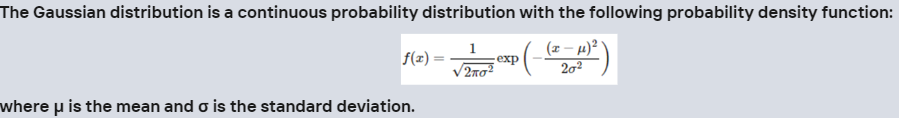
\includegraphics[width=\textwidth]{Images/1EpochQ1.png}
        \caption{Model trained on all of the data for one epoch}
        \label{fig: Q1_Model1}
    \end{subfigure}
    \hfill
    \begin{subfigure}[b]{0.5\textwidth}
        \centering
        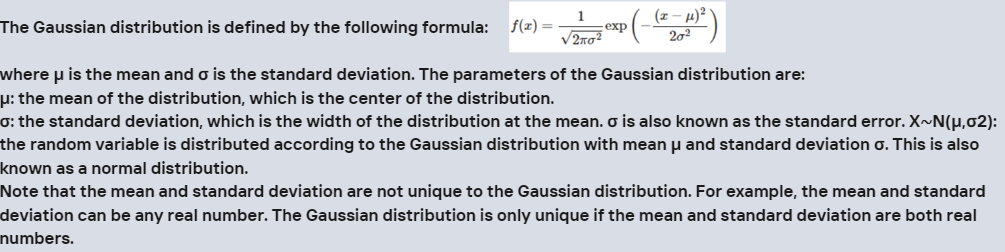
\includegraphics[width=\textwidth]{Images/10kQ1.png}
        \caption{Model trained on 10,000 observations for 3 epochs}
        \label{fig: Q1_Model2}
    \end{subfigure}
    \caption{Introductory level question : "\textit{What is the gaussian formula and all of its parameters?}"}
    \label{fig: Q1}
\end{figure}
From Figure \ref{fig: Q1_Model2}, we can see that the model trained on less data for more epochs
provided the exact same output as the model trained on more data for less epochs, seen
in Figure \ref{fig: Q1_Model1}, with a more in depth explanation of what each parameter
represents in the equation.

\begin{figure}[htbp]
    \centering
    \begin{subfigure}[b]{0.45\textwidth}
        \centering
        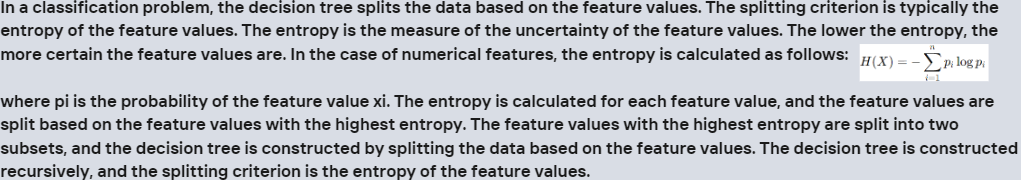
\includegraphics[width=\textwidth]{Images/1EpochQ2.png}
        \caption{Model trained on all of the data for one epoch}
        \label{fig: Q2_Model1}
    \end{subfigure}
    \hfill
    \begin{subfigure}[b]{0.5\textwidth}
        \centering
        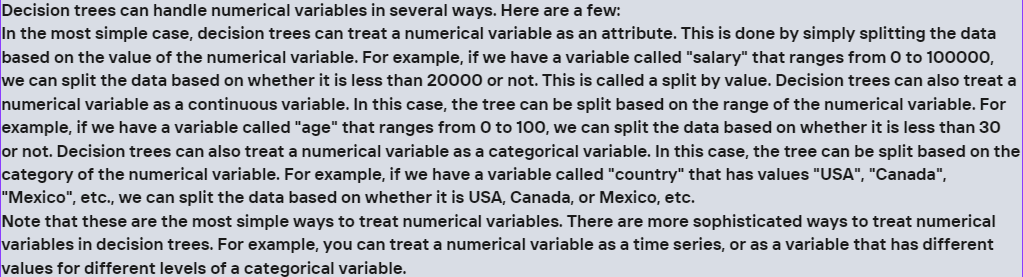
\includegraphics[width=\textwidth]{Images/10kQ2.png}
        \caption{Model trained on 10,000 observations for 3 epochs}
        \label{fig: Q2_Model2}
    \end{subfigure}
    \caption{Application level question : "\textit{Can you explain how decision trees handle numerical variables in a classification task?}"}
    \label{fig: Q2}
\end{figure}
From Figure \ref{fig: Q2_Model1} shows that model 1 provided a very good response
to the question, where \ref{fig: Q2_Model2} shows that the response from model
2 was also a good response on the questions and provided even more information
on how the decision tree handles categorical features when the tree is induced.

\begin{figure}[H]
    \centering
    \begin{subfigure}[b]{0.45\textwidth}
        \centering
        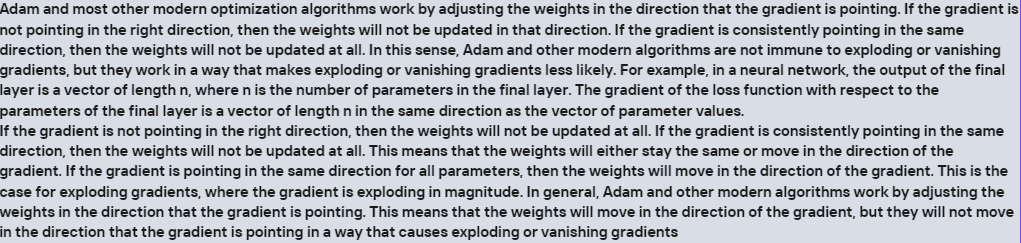
\includegraphics[width=\textwidth]{Images/1EpochQ3.png}
        \caption{Model trained on all of the data for one epoch}
        \label{fig: Q3_Model1}
    \end{subfigure}
    \hfill
    \begin{subfigure}[b]{0.5\textwidth}
        \centering
        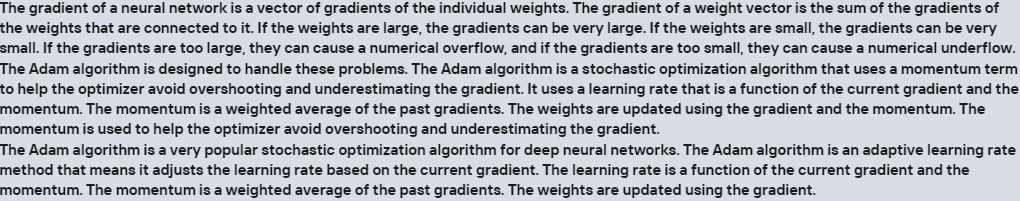
\includegraphics[width=\textwidth]{Images/10kQ3.png}
        \caption{Model trained on 10,000 observations for 3 epochs}
        \label{fig: Q3_Model2}
    \end{subfigure}
    \caption{Complex level question : "\textit{How do gradient-based optimization techniques like Adam handle exploding or vanishing gradient problems in deep learning models?}"}
    \label{fig: Q3}
\end{figure}
From Figure \ref{fig: Q3_Model1} and Figure \ref{fig: Q3_Model2} model 1 and model 2 respectively
gives a good response of the given question. Model 1 focuses more on the Adam optimiser and how
it handles exploding or vanishing gradients, where
model 2 focuses more on different techniques used by gradient-based optimisation techniques
to handle exploding and vanishing gradients.   

\section{Conclusion}

We have successfully scraped and wrangled data (from CrossValidated)
and used that data to fine-tune a 3 billion parameter LLaMa model.
After training 2 distinct models - one with a full epoch which uses all the
training data (39,686) and another with 3 epochs on 10,000 datapoints - on
Kaggle using their free 12 hour GPU sessions, we were able to get and run
inference on these large models and utilize their power.

Model 1 is able to give us broader answers to our related topics but lacks a
deeper understanding of the concepts whereas Model 2 is able to dive deeper
into the topics but is not able to discuss as many topics. 
Overall we prefer model 2 because it produces results that are
of higher understanding and complexity.

We are also able to locally run our models given the correct computer architecture. 
All in all we have successfully been able to create models that are capable of delivering
accurate and context aware responses to complex AI, machine learning, and data science questions.

\section{References}
\begin{thebibliography}{9}

\bibitem{llama3herd}
Meta AI Research. \textit{The LLaMA-3: Herd of Models}. Available at: \url{https://ai.meta.com/research/publications/the-llama-3-herd-of-models/}. Accessed: 2024-10-13.

\bibitem{unslothdocs}
Unsloth Documentation Team. \textit{Unsloth AI Documentation}. Available at: \url{https://docs.unsloth.ai/}. Accessed: 2024-10-13.

\bibitem{unslothfine-tune}
Unsloth AI Tutorials. \textit{How to Fine-Tune Llama 3 and Export to Ollama}. Available at: \url{https://docs.unsloth.ai/tutorials/how-to-finetune-llama-3-and-export-to-ollama}. Accessed: 2024-10-13.

\bibitem{stackexchange}
Stack Exchange Inc. \textit{Cross Validated - Statistical Analysis, Machine Learning, Data Mining, and Data Visualization}. Available at: \url{https://stats.stackexchange.com/}. Accessed: 2024-10-12.

\bibitem{stackexchange-tour}
Stack Exchange Inc. \textit{Cross Validated Tour: About}. Available at: \url{https://stats.stackexchange.com/tour#:~:text=Cross%20Validated%20is%20a%20question,Exchange%20network%20of%20Q\%26A\%20sites.}. Accessed: 2024-10-13.

\bibitem{googlesearch}
Google Search. \textit{Search Results: Cross Validated robots.txt}. Available at: \url{https://www.google.com/search?q=cross+validated+robots.txt&rlz=1C1GCEU_en-gbZA1068ZA1068&oq=cross+val}. Accessed: 2024-10-12.

\bibitem{beautifulsoup}
Richardson, Leonard. \textit{Beautiful Soup Documentation}. Available at: \url{https://pypi.org/project/beautifulsoup4/#:~:text=Beautiful%20Soup%20is%20a%20library,and%20modifying%20the%20parse%20tree.}. Accessed: 2024-10-13.

\bibitem{stackexchange-throttle}
Stack Exchange Inc. \textit{Throttle - Stack Exchange API Documentation}. Available at: \url{https://api.stackexchange.com/docs/throttle}. Accessed: 2024-10-23.

\bibitem{stackexchange-terms}
Stack Exchange Inc. \textit{Terms of Service - Stack Exchange}. Available at: \url{https://stats.stackexchange.com/legal/terms-of-service/public}. Accessed: 2024-10-12.

\end{thebibliography}


\end{document}
